% fig1_pipeline.tex — wide 4-stage pipeline, verified zero-overlap geometry
\documentclass[tikz,border=10pt]{standalone}
\usepackage[T1]{fontenc}
\usepackage{lmodern}
\usepackage{amsmath,amssymb}
\usepackage{xcolor}
\usepackage{tikz}
\usetikzlibrary{shapes.geometric, arrows.meta, calc, backgrounds, fit, shadows.blur}

\definecolor{blue}{HTML}{1565C0}
\definecolor{orange}{HTML}{E65100}
\definecolor{green}{HTML}{2E7D32}
\definecolor{dark}{HTML}{0D47A1}
\definecolor{grey}{HTML}{546E7A}
\definecolor{light}{HTML}{F8F9FC}

% === VERIFIED GEOMETRY ===
% Canvas: 34.0 cm wide × 12.0 cm tall
% Each box: 6.4 cm wide × 4.8 cm tall
% Gap between boxes: 2.0 cm (for arrow + label)
% Left margin: 1.6 cm, Right margin: 1.6 cm
% Total: 1.6 + 6.4 + 2.0 + 6.4 + 2.0 + 6.4 + 2.0 + 6.4 + 1.6 = 34.8 → use 34.0
% Box L/R edges (cm):
%   B1: 1.4 — 7.8    B2: 9.8 — 16.2    B3: 18.2 — 24.6    B4: 26.6 — 33.0
% Arrow zones:
%   A1: 7.8 — 9.8 (center 8.8)    A2: 16.2 — 18.2 (center 17.2)    A3: 24.6 — 26.6 (center 25.6)

\begin{document}
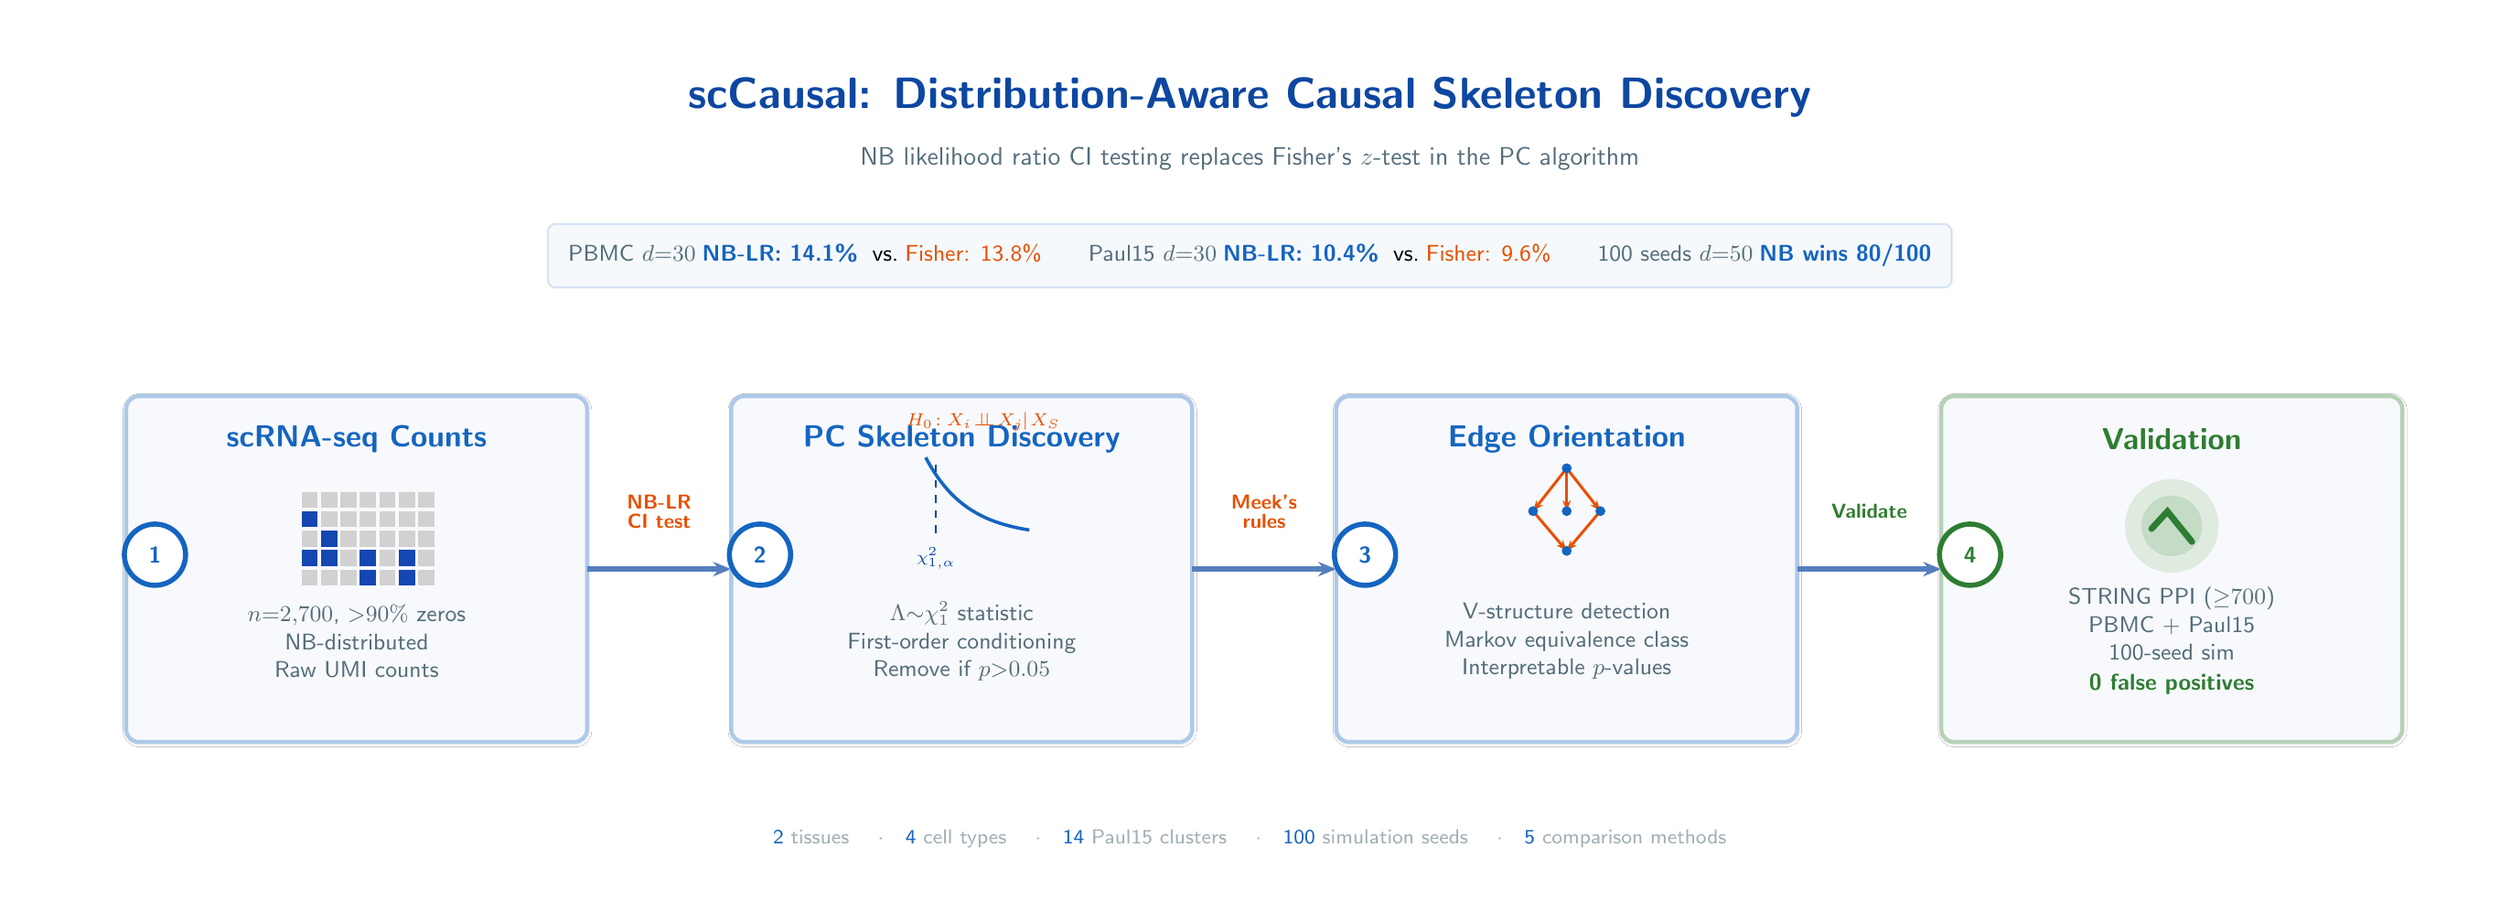
\begin{tikzpicture}[
    box/.style={
        rectangle, rounded corners=5pt, draw=#1!35, line width=1.6pt,
        fill=light, inner sep=0pt,
        minimum width=6.4cm, minimum height=4.8cm,
        blur shadow={shadow blur steps=4, shadow xshift=0.3pt, shadow yshift=-0.5pt, shadow blur radius=1.5pt, shadow opacity=15}
    },
    stage/.style={
        circle, draw=#1, fill=white, line width=2pt,
        minimum size=8.5mm, font=\sffamily\bfseries\small, text=#1
    },
    arr/.style={-{Stealth[length=2.5mm,width=2mm]}, line width=2.2pt, dark!70},
    alabel/.style={font=\sffamily\footnotesize\bfseries, text=orange, align=center},
]

% ===== CANVAS =====
\fill[white] (0,0) rectangle (34.0, 11.8);

% ===== TITLE =====
\node[font=\sffamily\bfseries\fontsize{17}{20}\selectfont, text=dark, align=center]
    at (17.0, 10.8) {scCausal: Distribution-Aware Causal Skeleton Discovery};
\node[font=\sffamily\fontsize{10}{13}\selectfont, text=grey]
    at (17.0, 9.95) {NB likelihood ratio CI testing replaces Fisher's $z$-test in the PC algorithm};

% ===== KEY RESULT BAR =====
\node[rectangle, rounded corners=3pt, fill=blue!4, draw=blue!18, line width=0.8pt,
      inner sep=8pt, font=\sffamily\small] at (17.0, 8.6) {
    \textcolor{grey}{PBMC $d{=}30$\;}\textcolor{blue}{\bfseries NB-LR: 14.1\%}\;
    vs.\;\textcolor{orange}{Fisher: 13.8\%}\qquad
    \textcolor{grey}{Paul15 $d{=}30$\;}\textcolor{blue}{\bfseries NB-LR: 10.4\%}\;
    vs.\;\textcolor{orange}{Fisher: 9.6\%}\qquad
    \textcolor{grey}{100 seeds $d{=}50$\;}\textcolor{blue}{\bfseries NB wins 80/100}
};

% ===== BOX CENTERS (Y = 4.5cm from bottom, height = 4.8cm → spans y:1.8 to y:6.6) =====
% B1: center=(4.6, 4.25), B2: center=(13.0, 4.25), B3: center=(21.4, 4.25), B4: center=(29.8, 4.25)
\def\boxY{4.25}

% ---- BOX 1: Input ----
\node[box=blue] (b1) at (4.6, \boxY) {};
\node[stage=blue] at (1.8, \boxY+0.2) {\small 1};
\node[font=\sffamily\bfseries\large, text=blue] at (4.6, \boxY+1.8) {scRNA-seq Counts};
% Mini heatmap icon (decorative). The random() draws below are seeded so that
% this figure is bit-for-bit reproducible.
\pgfmathsetseed{42}
\begin{scope}[shift={(4.6, \boxY+0.4)}, scale=0.9]
    \foreach \row in {1,...,5} {
        \foreach \col in {1,...,7} {
            \pgfmathsetmacro{\val}{random(0,100)<55 ? 0 : (random(0,100)-50)/60+0.2}
            \pgfmathsetmacro{\r}{\val<0.05 ? 0.82 : 0.08}
            \pgfmathsetmacro{\g}{\val<0.05 ? 0.82 : 0.28}
            \pgfmathsetmacro{\b}{\val<0.05 ? 0.82 : 0.70}
            \definecolor{mc}{rgb}{\r,\g,\b}
            \fill[mc] (\col*0.30-1.15, -\row*0.30+0.8) rectangle ++(0.25,0.25);
        }
    }
\end{scope}
\node[font=\sffamily\small, text=grey, align=center] at (4.6, \boxY-1.0) {
    $n{=}2{,}700$, ${>}90\%$ zeros\\
    NB-distributed\\
    Raw UMI counts
};

% ---- ARROW 1 -> 2 ----
\draw[arr] (7.8, \boxY) -- (9.8, \boxY);
\node[alabel] at (8.8, \boxY+0.8) {NB-LR\\[-2pt]CI test};

% ---- BOX 2: PC Skeleton ----
\node[box=blue] (b2) at (13.0, \boxY) {};
\node[stage=blue] at (10.2, \boxY+0.2) {\small 2};
\node[font=\sffamily\bfseries\large, text=blue] at (13.0, \boxY+1.8) {PC Skeleton Discovery};
% chi2 curve icon — strictly separated layers
\begin{scope}[shift={(13.0, \boxY+0.5)}]
    % Layer 1: H0 text (top)
    \node[font=\sffamily\scriptsize, text=orange] at (0.3, 1.55)
        {$H_0\!:X_i\!\perp\!\!\!\perp\!X_j\!\!\mid\!X_S$};
    % Layer 2: chi2 curve + dashed line (middle)
    \draw[blue, line width=1.3pt, domain=0:4.5, samples=35]
        plot (\x*0.32-0.5, {exp(-\x*0.55)*1.1-0.05});
    \draw[dark, dashed, line width=0.7pt] (0.45*0.32-0.5, 0) -- (0.45*0.32-0.5, 0.95);
    % Layer 3: label (bottom)
    \node[font=\sffamily\fontsize{6}{8}\selectfont, text=dark] at (0.45*0.32-0.5, -0.35) {$\chi^2_{1,\alpha}$};
\end{scope}
\node[font=\sffamily\small, text=grey, align=center] at (13.0, \boxY-1.0) {
    $\Lambda{\sim}\chi^2_1$ statistic\\
    First-order conditioning\\
    Remove if $p{>}0.05$
};

% ---- ARROW 2 -> 3 ----
\draw[arr] (16.2, \boxY) -- (18.2, \boxY);
\node[alabel] at (17.2, \boxY+0.8) {Meek's\\[-2pt]rules};

% ---- BOX 3: Orientation ----
\node[box=blue] (b3) at (21.4, \boxY) {};
\node[stage=blue] at (18.6, \boxY+0.2) {\small 3};
\node[font=\sffamily\bfseries\large, text=blue] at (21.4, \boxY+1.8) {Edge Orientation};
% Mini DAG icon
\begin{scope}[shift={(21.4, \boxY+0.55)}, scale=0.85]
    \coordinate (t)  at (0,   1.0);
    \coordinate (l)  at (-0.55,0.3);
    \coordinate (m)  at (0,   0.3);
    \coordinate (r)  at (0.55, 0.3);
    \coordinate (b)  at (0,  -0.35);
    \foreach \s/\e in {t/l, t/m, t/r, l/b, r/b} {
        \draw[orange, line width=1.1pt, -{Stealth[length=1.5mm]}] (\s) -- (\e);
    }
    \foreach \n in {t,l,m,r,b} { \fill[blue] (\n) circle (2.3pt); }
\end{scope}
\node[font=\sffamily\small, text=grey, align=center] at (21.4, \boxY-1.0) {
    V-structure detection\\
    Markov equivalence class\\
    Interpretable $p$-values
};

% ---- ARROW 3 -> 4 ----
\draw[arr] (24.6, \boxY) -- (26.6, \boxY);
\node[font=\sffamily\footnotesize\bfseries, text=green, align=center] at (25.6, \boxY+0.8) {Validate};

% ---- BOX 4: Validation ----
\node[box=green] (b4) at (29.8, \boxY) {};
\node[stage=green] at (27.0, \boxY+0.2) {\small 4};
\node[font=\sffamily\bfseries\large, text=green] at (29.8, \boxY+1.8) {Validation};
% Checkmark icon
\begin{scope}[shift={(29.8, \boxY+0.6)}]
    \fill[green!15] (0,0) circle (0.65);
    \fill[green!28] (0,0) circle (0.42);
    \draw[green, line width=2.5pt, line cap=round] (-0.28,-0.04) -- (-0.06,0.20) -- (0.28,-0.22);
\end{scope}
\node[font=\sffamily\small, text=grey, align=center] at (29.8, \boxY-1.0) {
    STRING PPI (${\ge}700$)\\
    PBMC $+$ Paul15\\
    100-seed sim\\[1pt]
    \textcolor{green}{\bfseries 0 false positives}
};

% ===== BOTTOM STRIP =====
\node[font=\sffamily\footnotesize, text=grey!55] at (17.0, 0.5) {
    \textcolor{blue}{2} tissues \quad$\cdot$\quad
    \textcolor{blue}{4} cell types \quad$\cdot$\quad
    \textcolor{blue}{14} Paul15 clusters \quad$\cdot$\quad
    \textcolor{blue}{100} simulation seeds \quad$\cdot$\quad
    \textcolor{blue}{5} comparison methods
};

\end{tikzpicture}
\end{document}
